% =====================================================================
%  ch03.tex —— 第 3 章 纤维丛（原书 p.28–44）
%  §3.1 定义  §3.2 主 G-丛  §3.3 向量丛  §3.4 向量丛与主 G-丛的联系
%  §3.5 切丛与余切丛  §3.6 定向与 spin 结构  §3.7 丛与标准模型
%  编号陈述 41 个（3.1–3.42，其中 3.16 在原书属 Fact，不在 statements.txt 的
%  类型表内）；另原书 Fact 3.16、3.43、3.44、3.45、3.46 共 5 个，用同一灰框体例。
%  编号公式 56 个（3.1–3.56）；图 3 张（fig3_1–fig3_3）。
% =====================================================================
\chapter{纤维丛}
\setcounter{footnote}{6}

% [原文 p.28]
看过一些流形的显式例子之后，我们转向纤维丛的研究。纤维丛是流形的一类扭曲的乘积。

\section{定义}

\begin{definition}{3.1}
纤维丛指的是这样一组数据：一个映射 $p:E\to B$，其中 $E$ 与 $B$ 是流形；并且存在一个固定的流形 $F$，使得对每个 $b\in B$，都有邻域 $b\in U\subset B$ 以及与投影相容的双射 $f:p^{-1}(U)\to U\times F$，即下图交换：
{\small
\[
\begin{array}{ccc}
p^{-1}(U) & \xrightarrow{\ f\ } & U\times F\\[3pt]
\big\downarrow & & \big\downarrow\\[3pt]
U & = & U
\end{array}
\tag{3.1}
\]
}
其中向下的箭头是投影。$F$、$E$、$B$ 分别称为纤维、全空间与底空间。上面的映射 $f$ 称为局部平凡化。
\end{definition}

换句话说，以 $F$ 为纤维、底空间为 $B$ 的纤维丛可以这样造：先用开集 $U_i$ 覆盖 $B$，对每个 $i$ 取乘积 $U_i\times F$，再在重叠 $U_{ij}:=U_i\cap U_j$ 上用映射 $f_{ij}$ 把它们粘起来：
{\small\setlength{\arraycolsep}{4pt}
\[
\begin{array}{ccccccc}
U_i\times F & \supset & U_{ij}\times F & \xrightarrow{\ f_{i,j}\ } & U_{ij}\times F & \subset & U_j\times F\\[3pt]
\downarrow & & \downarrow & & \downarrow & & \downarrow\\[3pt]
U_i & \supset & U_{ij} & = & U_{ij} & \subset & U_j
\end{array}
\tag{3.2}
\]
}
这里所有向下的箭头都是忘掉纤维方向的投影。

\begin{notation}{3.2}
为简便起见，我们常把一个纤维丛写成
\[
F \xrightarrow{\ \iota\ } E \xrightarrow{\ p\ } B.
\tag{3.3}
\]
其中 $\iota$ 是底空间 $B$ 中某点上方纤维的嵌入。
\end{notation}

在代数拓扑中，有一个更一般的概念叫纤维化，记号类似：$F\to E\to B$。纤维丛是纤维化，但纤维化不一定是纤维丛。

\begin{definition}{3.3}
两个有相同纤维的纤维丛 $F\to E\xrightarrow{p}B$ 与 $F\to E'\xrightarrow{p'}B$ 称为等价的，如果存在与投影相容的双射 $f:E\to E'$，即下图交换：
\[
\begin{array}{ccc}
E & \xrightarrow{\ f\ } & E'\\[3pt]
\downarrow & & \downarrow\\[3pt]
B & = & B
\end{array}
\tag{3.4}
\]
% [原文 p.29]
其中向下的箭头是投影 $p$ 与 $p'$。
\end{definition}

\begin{example}{3.4}
乘积 $E=B\times F$ 是以 $F$ 为纤维、底空间为 $B$ 的纤维丛。
\end{example}

\begin{center}
  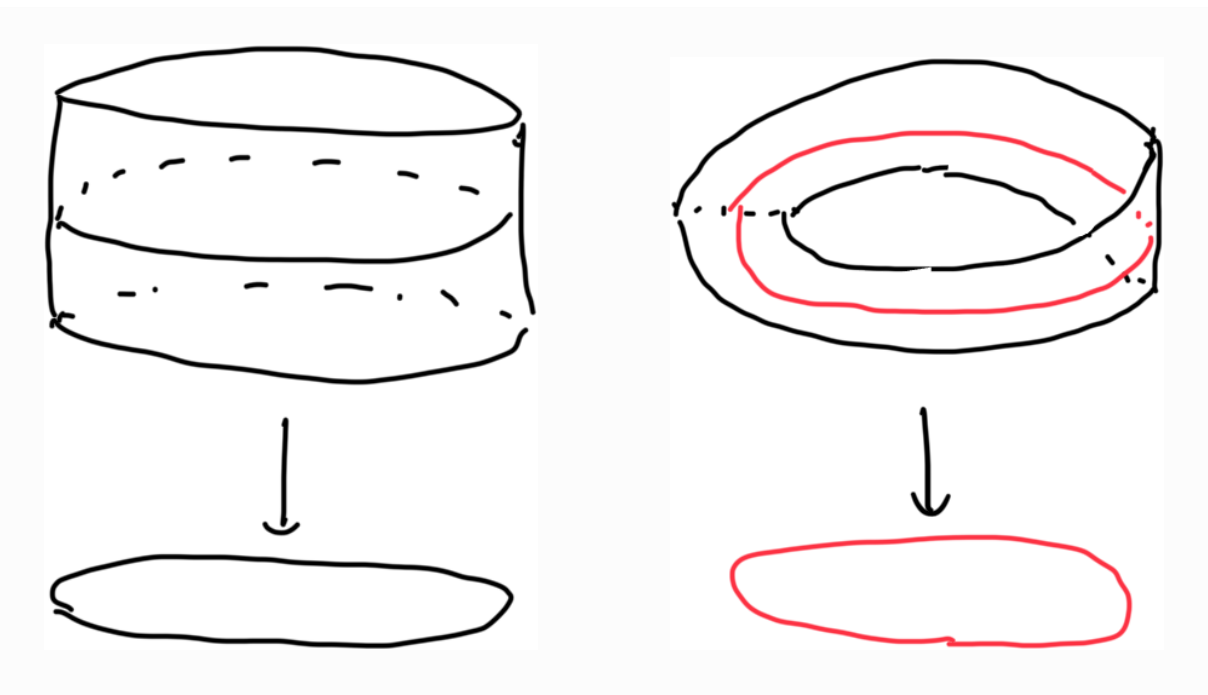
\includegraphics[width=0.62\textwidth]{figures/fig3_1.png}\\[2pt]
  {\small 图 3.1：柱面与 Möbius 带}
\end{center}

\begin{example}{3.5}
柱面 $S^1\times[-1,1]$ 是以 $[-1,1]$ 为纤维、底空间为 $S^1$ 的纤维丛。
\end{example}

\begin{example}{3.6}
Möbius 带是以 $S^1$ 为底空间、以线段 $[-1,1]$ 为纤维的纤维丛。
\end{example}

请看我画的这张糟糕的图，即图 3.1。

柱面与 Möbius 带是不等价的，尽管两者的纤维与底空间相同。看出这一点的一个办法，是注意柱面的边界是 $S^1\sqcup S^1$，而 Möbius 带的边界是 $S^1$。发展更一般的方法，去区分纤维相同、底空间也相同的不同纤维丛，正是纤维丛研究的目标之一。

\takeaway{本节给出纤维丛的定义：局部看是乘积 $U\times F$，整体由转移映射粘合。它比纤维化更特殊；而区分纤维与底空间都相同的不同丛，正是本学科的目标之一。}

\section{主 $G$-丛}

\subsection{一般情形}

\begin{proposition}{3.7}
设 $G$ 作用在流形 $M$ 上。再设这个作用是自由的，即对每个 $m\in M$，满足 $mg=m$ 的 $g\in G$ 只有 $g=e$。那么投影 $p:M\to M/G$ 是以 $G$ 为纤维的纤维丛。换言之，我们有一个纤维丛
\[
G\to M\to M/G.
\]
\end{proposition}

在这个描述里，可以说我们让全空间 $M$ 比底空间 $M/G$ 更重要。若改以底空间 $B=M/G$ 为主要对象，就得到下面的观点：

% [原文 p.30]
\begin{definition}{3.8}
以 $G$ 为纤维的纤维丛 $p:P\to B$ 称为主 $G$-丛（principal $G$-bundle），如果 $P$ 上配有 $G$ 的右作用，使得对每个 $b\in B$ 都有 $U\subset B$，并且有与 $G$ 作用相容的如下等同：
{\small
\[
\begin{array}{ccc}
p^{-1}(U) & \simeq & U\times G\\[3pt]
\big\downarrow & & \big\downarrow\\[3pt]
U & = & U
\end{array}.
\tag{3.5}
\]
}
\end{definition}

现在，全空间 $P$ 像前面那样，通过把 $U_i\times G$ 与 $U_j\times G$ 在 $U:=U_i\cap U_j$ 上粘起来而得到：
{\small\setlength{\arraycolsep}{4pt}
\[
\begin{array}{ccccccc}
U_i\times G & \supset & U\times G & \xrightarrow{\ f_{ij}\ } & U\times G & \subset & U_j\times G\\[3pt]
\downarrow & & \downarrow & & \downarrow & & \downarrow\\[3pt]
U_i & \supset & U & = & U & \subset & U_j
\end{array}
\tag{3.6}
\]
}
其中 $f_{ij}$ 必须与 $G$ 的右作用相容。我们来把 $f_{ij}$ 写得更显式。

为此需要下面这个同义反复式的引理：

\begin{lemma}{3.9}
与右 $G$ 作用相容的映射 $f:G\to G$，由某个元素 $g\in G$ 的左乘给出，即 $f(h)=gh$。
\end{lemma}

确实，我们需要 $f(h_1h_2)=f(h_1)h_2$。因此 $f(h)=f(eh)=f(e)h$。令 $g:=f(e)$，就有 $f(h)=gh$。证毕。

在每个点 $b\in U$ 上使用这个引理，可以看出 $f_{ij}:U\times G\to U\times G$ 由某个函数 $g_{ij}:U\to G$ 显式地给出：
\[
f_{ij}:(b,g)\mapsto(b,g_{ij}(b)g).
\tag{3.7}
\]

主 $G$-丛 $P\to B$ 何时与平凡丛 $B\times G\to B$ 等价？按定义，这意味着存在与投影以及右 $G$ 作用都相容的双射 $h:P\to B\times G$。在每个片 $U_i$ 上，$h$ 由与 $G$ 作用及投影都相容的 $f'_i:p^{-1}(U_i)\to U_i\times G$ 给出。再次使用上面的引理，它由映射 $g'_i:U_i\to G$ 决定，即 $f'_i(b,g)=(b,g'_i(b)g)$。此外，这些 $g'_i$ 必须与粘合过程相容，也就是说下图必须交换：
\[
\begin{array}{ccc}
G & \xrightarrow{\ g_{ij}\ } & G\\[3pt]
{\scriptstyle g'_i}\big\downarrow & & \big\downarrow{\scriptstyle g'_j}\\[3pt]
G & \xrightarrow{\ \id\ } & G,
\end{array}
\tag{3.8}
\]
即 $g_{ij}=(g'_j)^{-1}g'_i$。总结起来，我们得到：

\begin{proposition}{3.10}
用式 (3.7) 给出的主 $G$-丛 $P\to B$，与平凡主 $G$-丛 $B\times G\to B$ 等价，当且仅当存在映射 $g_i:U_i\to G$ 使得 $g_{ij}=(g_j)^{-1}g_i$。
\end{proposition}

\subsection{例子}

% [原文 p.31]
现在，§2.4 中见过的许多例子都可以改述为主丛。特别地，命题 2.32 意味着：

\begin{example}{3.11}
$S^n\to\RP^n$ 是主 $O(1)=\Z_2$-丛。
\end{example}

\begin{example}{3.12}
$S^{2n+1}\to\CP^n$ 是主 $U(1)=S^1$-丛。
\end{example}

\begin{example}{3.13}
$S^{4n+3}\to\HP^n$ 是主 $Sp(1)=SU(2)=S^3$-丛。
\end{example}

此外，我们在式 (2.39) 中看到 $\RP^1=S^0$、$\CP^1=S^2$、$\HP^1=S^3$。这意味着我们有下列纤维丛：
\begin{itemize}
  \item $\R^2\supset S^1\to\RP^1=S^1$ 是 $S^0$ 丛，
  \item $\C^2\supset S^3\to\CP^1=S^2$ 是 $S^1$ 丛，
  \item $\mathbb{H}^2\supset S^7\to\HP^1=S^4$ 是 $S^3$ 丛。
\end{itemize}
这些称为 Hopf 纤维化。它们是非平凡的，与乘积不同。例如在第二种情形，全空间是 $S^3$，它不同于 $S^2\times S^1$，即 $S^2$ 上平凡 $S^1$ 丛的全空间。（注意我们其实还没学过如何区分 $S^3$ 与 $S^1\times S^2$。这件事以后再做。）

% [体例] 原书 p.31：Remark 3.14 为无框斜体段、段末右下角 ⌟（preamble 的 remark 环境已是无框正文，段末自动加 \qedmark）。
\begin{remark}{3.14}
第一个例子是 2:1 的映射，已经在图 3.1 中画成从 Möbius 带的边界 $S^1$ 到底空间 $S^1$ 的映射。
\end{remark}

% [体例] 原书 p.31–p.32：Remark 3.15 同为无框斜体段，⌟ 在 p.32 段末（preamble 的 remark 环境自动加）。
\begin{remark}{3.15}
第二个例子可以换一种描述。把 $S^3$ 看作一个量子比特中范数为 1 的态的参数空间：
\[
\ket{\psi}=\begin{pmatrix}u\\,\qquad (|u|^2+|v|^2=1).
\tag{3.9}
\]
现在取 Pauli 矩阵的期望值：
\begin{align}
x&:=\bra{\psi}\sigma_X\ket{\psi}=\bar u v+\bar v u,\tag{3.10}\\
y&:=\bra{\psi}\sigma_Y\ket{\psi}=-i\bar u v+i\bar v u,\tag{3.11}\\
z&:=\bra{\psi}\sigma_Z\ket{\psi}=|u|^2-|v|^2.\tag{3.12}
\end{align}
容易验证 $x^2+y^2+z^2=1$。因此映射
\[
(u,v)\mapsto(x,y,z)
\tag{3.13}
\]
% [原文 p.32]
定义了一个映射
\[
S^3\to S^2.
\tag{3.14}
\]
这个映射的纤维是 $S^1$，这一点从期望值在变换 $\ket{\psi}\mapsto c\ket{\psi}$（其中 $|c|=1$）下不变即可看出。由 $(x,y,z)$ 参数化的球面 $S^2$，常被称为该量子比特的 Bloch 球面。\footnote{这个术语背后的历史相当有趣。它源自 [ACGT72] 一篇关于量子光学的论文，作者们在其中引用了 Felix Bloch 关于核磁共振的工作 [Blo46]；不过 Bloch 的这篇论文根本没有研究我们今天所知的 Bloch 球面。此后这个术语被量子信息学界采用，又因量子比特日益流行而成为更普遍的通用术语。（我用了 \url{https://physics.stackexchange.com/questions/636913/} 作为来源。）} 我们也可以给上面的映射一个更显式的参数化：
\[
(\cos(\theta/2)e^{i\psi},\ \sin(\theta/2)e^{i(\phi+\psi)})\mapsto(\sin\theta\cos\phi,\ \sin\theta\sin\phi,\ \cos\theta).
\tag{3.15}
\]
这说明 $S^2$ 上一点上方的纤维由 $\psi$ 参数化。

我们可以通过
\[
(a,b,c,d)\mapsto\frac{1}{1-a}(b,c,d)
\tag{3.16}
\]
把 $S^3$ 上的点球极投影到 $\R^3$，见图 3.2。利用这个投影，可以把 $S^2$ 上每一点的纤维画成 $\R^3$ 中的圆。在图 3.3 中，我就用这种方式画出了 $(\cos 2\pi k/8,\ \sin 2\pi k/8,\ 0)$（$k=0,1,\dots,7$）的纤维。
\end{remark}

\begin{center}
  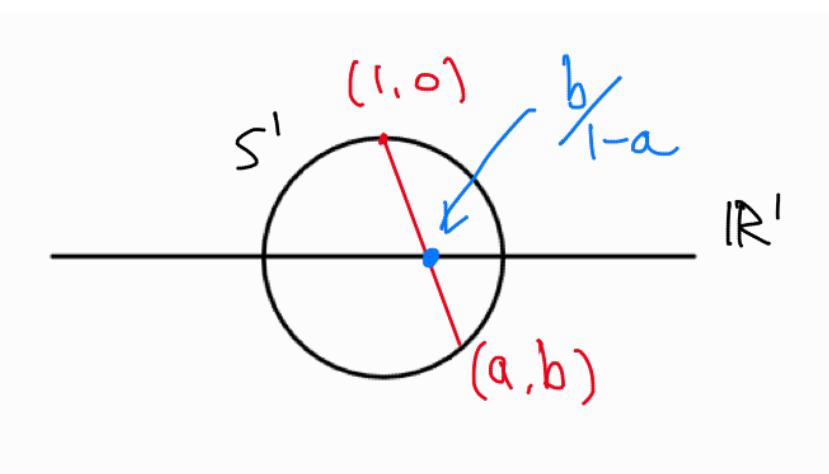
\includegraphics[width=0.58\textwidth]{figures/fig3_2.png}\\[2pt]
  {\small 图 3.2：$S^3$ 到 $\R^3$ 的球极投影}
\end{center}

注意，上面三个纤维化都有 $S^n\to S^m\to S^{m-n}$ 的形式。人们会问，这种形式的例子还有没有别的。其实有：

\begin{qmbox}
\qmstmt{事实}{3.16} 这三个 Hopf 纤维化，再加上最后一个 $S^7\to S^{15}\to S^8$，穷尽了这种形式的纤维化 $S^n\to S^m\to S^{m-n}$。
\end{qmbox}

最后这个与八元数有关，它不是主纤维丛，因为 $S^7$ 不是群。

我们还可以利用 Hopf 纤维化非平凡这一点，来说明例 3.11、3.12、3.13 给出的纤维化全都非平凡。下面以 $\RP^n$ 的情形示范。为此考虑下图：
{\small
\[
\begin{array}{ccccc}
\Z_2 & \to & S^n & \to & \RP^n\\
\| & & \cup & & \cup\\
\Z_2 & \to & S^1 & \to & \RP^1.
\end{array}
\tag{3.17}
\]
}

% [原文 p.33]
\begin{center}
  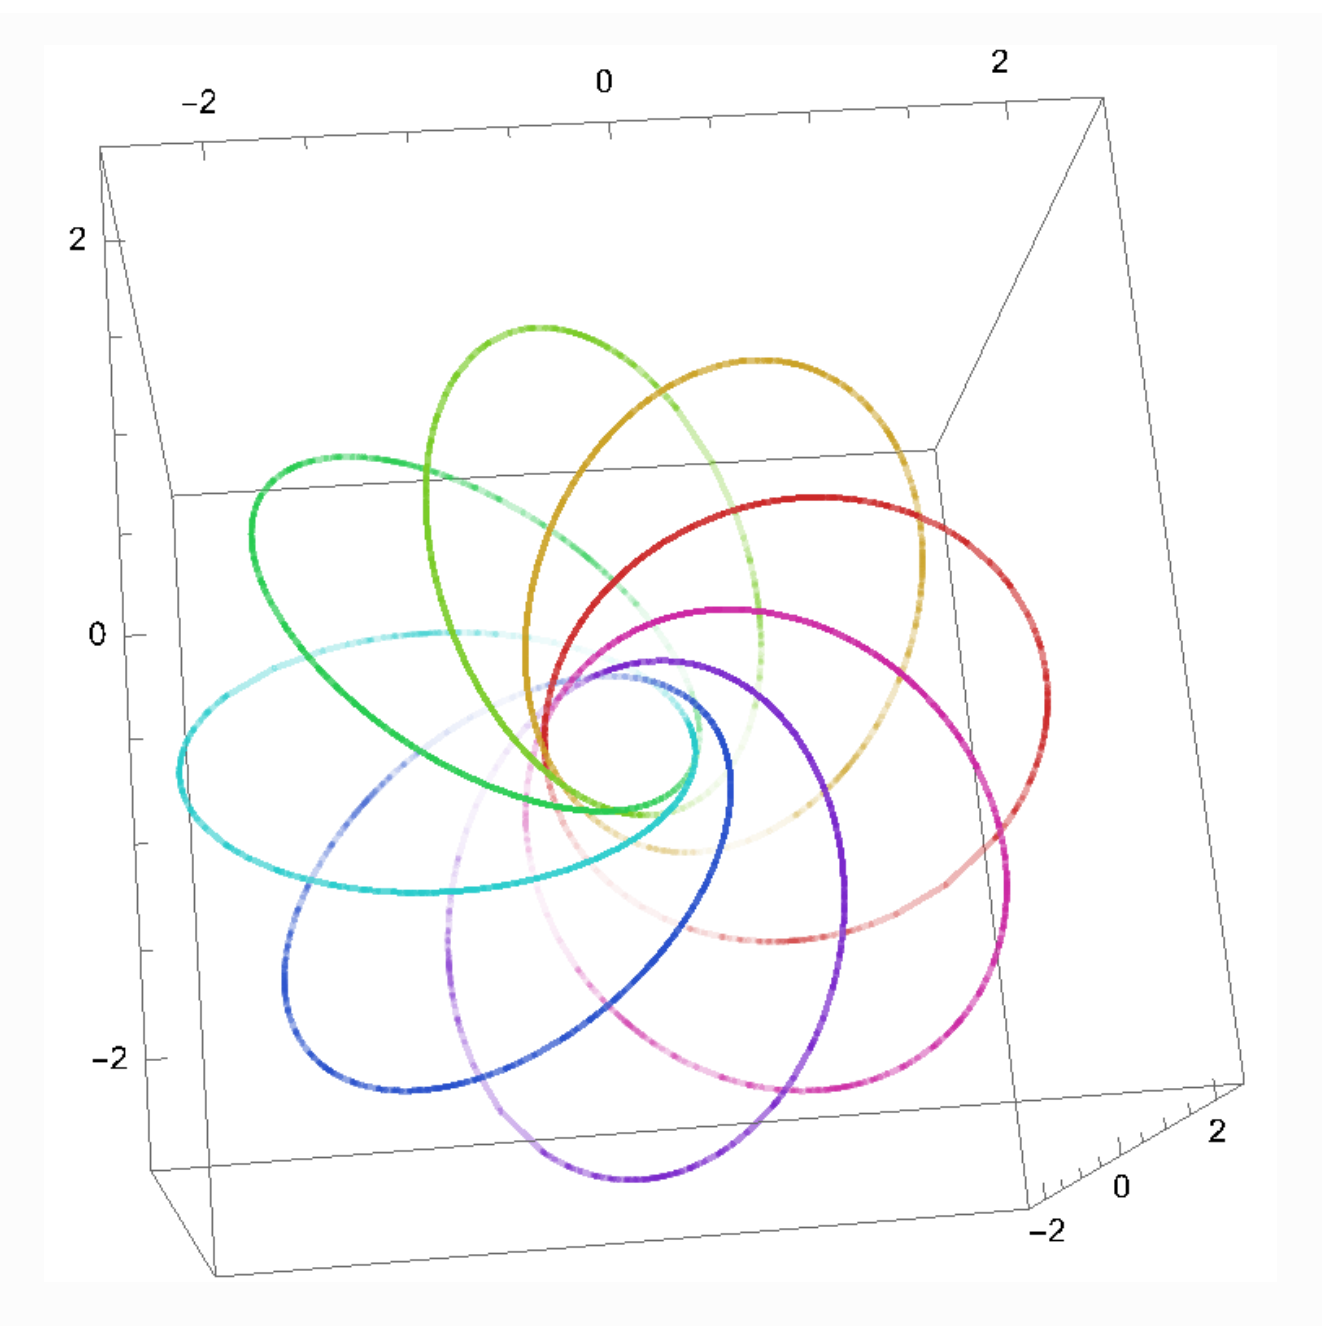
\includegraphics[width=0.55\textwidth]{figures/fig3_3.png}\\[2pt]
  {\small 图 3.3：经球极投影画出的 Hopf 纤维化的纤维}
\end{center}

这里 $S^1\subset S^n$ 是把大部分坐标限制为零得到的。我们已经看到第二行是非平凡纤维化。第一行包含第二行，所以第一行也非平凡。总结一下，我们有：

\begin{proposition}{3.17}
纤维化 $\Z_2\to S^n\to\RP^n$、$S^1\to S^{2n+1}\to\CP^n$、$S^3\to S^{4n+3}\to\HP^n$ 都非平凡。
\end{proposition}

在定义 2.34 中引入、并在其下给了许多例子的齐性空间，也给出主丛。

\begin{proposition}{3.18}
$G$ 是 $G/H$ 上的主 $H$-丛，即我们有纤维丛 $H\to G\to G/H$。
\end{proposition}

我们给出一个 §2.4.3 中没有直接处理的例子。考虑 $g\in SU(2)$ 作用在 $\C^2$ 上。注意 $2\times2$ 的无迹 Hermite 矩阵由 $\R^3$ 参数化，即 $x\sigma_x+y\sigma_y+z\sigma_z$。我们让 $g\in SU(2)$ 通过
\[
R_g:(x,y,z)\mapsto(x',y',z')
\tag{3.18}
\]
作用在这个空间上，其中
\[
g(x\sigma_x+y\sigma_y+z\sigma_z)g^\dagger=x'\sigma_x+y'\sigma_y+z'\sigma_z.
\tag{3.19}
\]
在这个 $SU(2)$ 作用下不变的函数 $V:\R^3\to\R$ 具有 $V(x,y,z)=f(r)$ 的形式，其中 $r^2=x^2+y^2+z^2$。设 $f(r)$ 在 $r_0>0$ 处取极小值。则势的极小值空间是 $x^2+y^2+z^2=r_0^2$，它是一个球面 $S^2$。

% [原文 p.34]
取 $m_0=(0,0,r_0)$，它对应 $r_0\sigma_z$。固定这个点的 $SU(2)\simeq S^3$ 的元素具有 $e^{i\theta\sigma_z}$ 的形式（$\theta$ 为某个值），它同构于 $U(1)\simeq S^1$。这样我们又得到了
\[
S^1\to S^3\to S^2.
\tag{3.20}
\]

这个对称破缺模式最早由 Georgi 与 Glashow 在电弱理论的背景下引入 [GG72]。虽然它与实验结果不符，但仍可充当比真实情形（标准模型）更简单的模型，供我们练习技巧。它在我们后面分析磁单极子时也会起重要作用。

注意，我们通过 $g\mapsto R_g$ 定义了一个映射 $SU(2)\to SO(3)$，其中 $R_g$ 由式 (3.18) 与式 (3.19) 给出。这是一个同态，核为 $\{\pm1\}$。换句话说，我们得到：

\begin{example}{3.19}
存在纤维丛 $\{\pm1\}\to SU(2)\to SO(3)$。
\end{example}

回想起 $SU(2)\simeq S^3$，我们还看出

\begin{proposition}{3.20}
$SO(3)\simeq\RP^3$。
\end{proposition}

注意，这不过是纤维化 $\Z_2\to S^n\to\RP^n$ 在 $n=3$ 时的例子，因此它非平凡，正如我们在命题 3.17 中已经看到的。

\takeaway{主 $G$-丛是带右作用的纤维丛，转移函数由 $g_{ij}:U\to G$ 给出，平凡性判据是 $g_{ij}=(g_j)^{-1}g_i$。Hopf 纤维化与齐性空间是典型例子，并由此得到 $\SO(3)\simeq\RP^3$。}

\section{向量丛}

另一大类丛是向量丛，其纤维是向量空间。

\begin{definition}{3.21}
取标量域 $\mathbb{K}$ 为 $\R$、$\C$ 或 $\mathbb{H}$。向量丛是以 $V$ 为纤维的纤维丛 $E\to B$，其中 $V$ 是向量空间，并且 $U_i\subset B$ 与 $U_j\subset B$ 上的两个局部平凡化在重叠 $U:=U_i\cap U_j$ 上按如下方式相联系：
{\small\setlength{\arraycolsep}{4pt}
\[
\begin{array}{ccccccc}
U_i\times V & \supset & U\times V & \xrightarrow{\ f\ } & U\times V & \subset & U_j\times V\\[3pt]
\downarrow & & \downarrow & & \downarrow & & \downarrow\\[3pt]
U_i & \supset & U & = & U & \subset & U_j
\end{array}
\tag{3.21}
\]
}
其中 $f$ 由
\[
f:(b,v)\mapsto(b,g(b)v)
\tag{3.22}
\]
给出，而 $g(b):V\to V$ 是依赖于 $b\in U$ 的光滑线性映射。$V$ 的维数称为该向量丛的秩。
\end{definition}

$\R$-向量丛、$\C$-向量丛、$\mathbb{H}$-向量丛也分别称为实、复、四元数向量丛。

在物理中，向量丛的纤维 $V$ 上常常还有内积，于是转移函数 $g(b)$ 不只是线性映射，而是分别属于 $O(n)$、$U(n)$ 或 $Sp(n)$。这一点以后再回来讨论。

% [原文 p.35]
\begin{definition}{3.22}
向量丛 $p:E\to B$ 的截面是一个映射 $\psi:B\to E$，使得 $p\circ\psi$ 是 $B$ 上的恒等映射。
\end{definition}

更不正式地说，$\psi(b)$（$b\in B$）取值于 $b$ 上方的纤维 $V$ 中。向量丛的截面在物理中通常以两种方式之一出现：
\begin{itemize}
  \item 作为场：底空间 $B$ 是时空，纤维 $V$ 是场可以取的值的集合。这在 hep-th 的规范理论背景中无处不在。广义相对论中的度规张量也是某个向量丛的截面。
  \item 作为量子力学系统的波函数：系统可以分解为沿底空间 $B$ 的自由度，以及由纤维 $V$ 参数化的额外自由度，$V$ 是某个量子子系统的希尔伯特空间。例如在 Born--Oppenheimer 近似中就出现这种情况：$B$ 对应某些自由度（如原子核的位置）的慢运动，$V$ 对应另一些自由度（如电子）的快运动。在研究晶体材料时也会出现：此时 $B$ 是布里渊区，$V$ 是固定波数处量子态构成的空间。
\end{itemize}

\begin{definition}{3.23}
纤维在 $\mathbb{K}$ 上是一维的向量丛称为 $\mathbb{K}$-线丛。这里 $\mathbb{K}$ 是 $\R$、$\C$ 或 $\mathbb{H}$。
\end{definition}

大多数时候，线丛指的是复线丛，即纤维为一维复向量空间的向量丛。\footnote{我觉得数学家有点疯，居然把复数构成的空间叫作“线”。}

当我们有两个向量空间 $V$ 与 $W$ 时，可以作直和 $V\oplus W$ 或张量积 $V\otimes W$。这些运算可以逐纤维地进行，从而提升到向量丛上。

\begin{definition}{3.24}
给定纤维为 $V$ 与 $W$ 的两个向量丛 $E\to B$ 与 $E'\to B$，我们可以作 $B$ 上纤维为 $V\oplus W$ 的直和 $E\oplus E'$，或 $B$ 上纤维为 $V\otimes W$ 的张量积丛 $E\otimes E'$。
\end{definition}

给定向量空间 $V$，线性函数 $V\to\mathbb{K}$ 构成的空间记为 $V^*$，它也是向量空间。逐纤维地做这件事，就有：

\begin{definition}{3.25}
给定纤维为 $V$ 的向量丛 $E\to B$，我们可以作纤维为 $V^*$ 的对偶丛 $E^*\to B$。
\end{definition}

类似地，对于复向量丛，我们可以做：

\begin{definition}{3.26}
给定纤维为 $V$ 的复向量丛 $E\to B$，我们可以作纤维为 $\ol{V}$ 的复共轭丛 $\ol{E}\to B$。
\end{definition}

还可以做另一个有趣的操作。设 $V$ 是带 Hermite 内积的复向量空间。令 $\operatorname{Herm}(V)$ 为 $V$ 上 Hermite 算子构成的空间，它是一个实向量空间。

% [原文 p.36]
\begin{definition}{3.27}
给定纤维为 $V$ 的复向量丛 $E\to B$，我们可以作纤维为 $\operatorname{Herm}(V)$ 的 Hermite 算子丛 $\operatorname{Herm}(E)\to B$。
\end{definition}

给定在参数空间 $B$ 上参数化的一族希尔伯特空间，这个操作给出同一参数空间 $B$ 上的一族空间：对每个希尔伯特空间，取作用于其上的可观测量所构成的空间。

还可以逐纤维地做另一种不同的操作：在每条纤维上取单位球面 $\operatorname{Sph}(V)=S^{kn-1}\subset V$，其中 $n$ 是 $V$ 的维数，$k=1,2,4$ 分别对应 $\mathbb{K}=\R,\C,\mathbb{H}$。

\begin{definition}{3.28}
给定纤维为 $V$ 的向量丛 $E\to B$，我们可以作纤维为 $\operatorname{Sph}(V)$ 的球丛 $\operatorname{Sph}(E)\to B$。
\end{definition}

我们也可以考虑在每条纤维上取向量子空间 $V_2\subset V_1$：

\begin{definition}{3.29}
纤维为 $V_1$ 的向量丛 $E_1\to B$ 的子丛，是纤维为 $V_2$ 的向量丛 $E_2\to B$，使得在每个局部平凡化上都有
{\small\setlength{\arraycolsep}{4pt}
\[
\begin{array}{ccccccc}
(p_2)^{-1}(B) & \simeq & U\times V_2 & \subset & U\times V_1 & \simeq & (p_1)^{-1}(B)\\[3pt]
\downarrow & & \downarrow & & \downarrow & & \downarrow\\[3pt]
U & = & U & = & U & = & U
\end{array}
\tag{3.23}
\]
}
\end{definition}

我们来看一个基本而有趣的例子。考虑单位球面 $S^2$，用满足 $x^2+y^2+z^2=1$ 的 $(x,y,z)$ 参数化。考虑 $S^2$ 上的平凡向量丛 $S^2\times\mathcal{H}$，其中 $\mathcal{H}=\C^2$ 是一个量子比特。考虑在 $S^2$ 上参数化的 Hamilton 量
\[
H:=-(x\sigma_x+y\sigma_y+z\sigma_z).
\tag{3.24}
\]
由于 $H^2=1$，$H$ 的本征值为 $\pm1$。令 $V(x,y,z)\subset\mathcal{H}$ 为最低能量的本征空间，即 $-1$ 本征空间。这确定了平凡丛 $S^2\times\mathcal{H}$ 在 $S^2$ 上的一个子丛 $E\to S^2$，其中 $(x,y,z)$ 处的纤维是 $V(x,y,z)$。这是一个复线丛。

为了更显式地描述这个丛，让我们回忆从 $S^3$ 到 $S^2$ 的映射 (3.13)，并用 $(u,v)$ 表示 $(x,y,z)$。容易验证
\[
H\begin{pmatrix}u\\
=-\begin{pmatrix}|u|^2-|v|^2 & 2\bar v u\\[2pt] 2\bar u v & -|u|^2+|v|^2\end{pmatrix}
\begin{pmatrix}u\\
=-\begin{pmatrix}u\\
\tag{3.25}
\]
我们证明了
\[
V(x,y,z)=\Bigl\{c\begin{pmatrix}u\\ \Big|\ c\in\C\Bigr\}\subset\mathcal{H}.
\tag{3.26}
\]
现在可以取单位球丛 $\operatorname{Sph}(E)\to S^2$。它把满足 $|u|^2+|v|^2=1$ 的 $(u,v)$ 经式 (3.13) 送到 $(x,y,z)$，所以这就是 Hopf 纤维化 $S^1\to S^3\to S^2$。总结一下：

% [原文 p.37]
\begin{example}{3.30}
$S^2$ 上复线丛的单位球丛——该复线丛由 Hamilton 量 (3.24) 的最低能量态得到——是 Hopf 纤维化 $S^1\to S^3\to S^2$。
\end{example}

\takeaway{向量丛的纤维是向量空间，转移函数逐点线性。截面、线丛、直和、张量积、对偶、共轭、球丛与子丛都逐纤维构造；$S^2$ 上 Hamilton 量 (3.24) 的最低能态给出 Hopf 丛。}

\section{向量丛与主 $G$-丛的联系}

我们在式 (3.22) 中描述了向量丛的转移函数。在完全一般的复向量丛 $E\to B$ 上，转移函数 $g(b)$ 属于 $GL(n,\C)$，其中 $n$ 是该向量丛的秩，即纤维的维数。但我们常考虑向量丛的纤维配有 Hermite 内积的情形。这时转移函数属于 $U(n)$。于是可以按式 (3.7) 定义与该向量丛相伴的主 $U(n)$-丛 $P\to B$。此时纤维不再是 $\C^n$，而是 $U(n)$。

在高能物理中，我们常遇到 $g(b)$ 落在 $U(n)$ 的某个子群 $G$ 中的情形；这时可以同样地考虑与该向量丛相伴的主 $G$-丛。此时纤维不再是 $\C^n$，而是 $G$。

\begin{definition}{3.31}
若 $\mathbb{K}$-向量丛的转移函数 $g(b)$ 落在 $GL(n,\mathbb{K})$ 的某个子群 $G$ 中，则称该向量丛具有结构群 $G$。由同一组转移函数给出的主 $G$-丛，称为该向量丛的相伴主 $G$-丛。
\end{definition}

还有反向的操作。取 $B$ 上一个主 $G$-丛，其在 $U:=U_i\cap U_j$ 上的转移函数由映射 $g:U\to G$ 按式 (3.7) 给出。取 $G$ 在向量空间 $V$ 上的一个线性作用 $\rho:G\curvearrowright V$。于是可以这样定义 $B$ 上纤维为 $V$ 的向量丛：规定其 $U_i\times V$ 与 $U_j\times V$ 之间的转移函数由 $\rho(g)$ 给出，即
{\small\setlength{\arraycolsep}{4pt}
\[
\begin{array}{ccccccc}
U_i\times V & \supset & U\times V & \xrightarrow{\ f\ } & U\times V & \subset & U_j\times V\\[3pt]
\downarrow & & \downarrow & & \downarrow & & \downarrow\\[3pt]
U_i & \supset & U & = & U & \subset & U_j
\end{array}
\tag{3.27}
\]
}
其中 $f$ 由
\[
f:(b,v)\mapsto(b,\rho(g(b))v)
\tag{3.28}
\]
给出。

\begin{definition}{3.32}
如上构造出的向量丛 $V\to E\to B$，称为主 $G$-丛 $G\to P\to B$ 的相伴向量丛，由表示 $\rho$ 决定。我们称 $G$ 为 $E\to B$ 的结构群。
\end{definition}

作为例子，取主 $U(1)$-丛 $U(1)\to E\to B$：
{\small\setlength{\arraycolsep}{4pt}
\[
\begin{array}{ccccccc}
U_i\times U(1) & \supset & U\times U(1) & \xrightarrow{\ f\ } & U\times U(1) & \subset & U_j\times U(1)\\[3pt]
\downarrow & & \downarrow & & \downarrow & & \downarrow\\[3pt]
U_i & \supset & U & = & U & \subset & U_j
\end{array}
\tag{3.29}
\]
}
其中 $f$ 由
\[
f:(b,h)\mapsto(b,g(b)h)
\tag{3.30}
\]
% [原文 p.38]
给出，这里 $b\in B$、$h\in U(1)$（即 $|h|=1$）、$g:U\to U(1)$。取 $U(1)$ 在 $\C$ 上由乘法给出的标准表示，即 $g\in U(1)$ 通过 $z\mapsto gz$ 作用在 $z\in\C$ 上。则相伴向量丛 $\C\to E'\to B$ 具有结构
{\small\setlength{\arraycolsep}{4pt}
\[
\begin{array}{ccccccc}
U_i\times\C & \supset & U\times\C & \xrightarrow{\ f'\ } & U\times\C & \subset & U_j\times\C\\[3pt]
\downarrow & & \downarrow & & \downarrow & & \downarrow\\[3pt]
U_i & \supset & U & = & U & \subset & U_j
\end{array}
\tag{3.31}
\]
}
其中 $f$ 由
\[
f':(b,z)\mapsto(b,g(b)z)
\tag{3.32}
\]
给出，$z\in\C$。容易看出 $E\to B$ 是 $E'\to B$ 的单位球丛。总结一下，我们得到：

\begin{proposition}{3.33}
给定主 $U(1)$-丛 $U(1)\to E\to B$，考虑由标准表示 $U(1)\curvearrowright\C$ 得到的相伴向量丛 $\C\to E'\to B$。那么 $E\to B$ 是 $E'\to B$ 的单位球丛。
\end{proposition}

我们在例 3.30 中看到，$S^2$ 上 Hamilton 量 (3.24) 最低能量态的复线丛，其单位球丛是 Hopf 纤维化 $S^1\to S^3\to S^2$。因此反过来，Hopf 纤维化 $S^1\to S^3\to S^2$ 在标准表示 $U(1)\curvearrowright\C$ 下的相伴线丛，就是 Hamilton 量 (3.24) 最低能量态的复线丛。

不用片而构造相伴向量丛的另一种方式如下。

\begin{proposition}{3.34}
给定主 $G$-丛 $G\to P\to B$ 与表示 $\rho:G\curvearrowright V$，相伴向量丛 $V\to E\to B$ 由 $E=(P\times V)/G$ 给出，其中 $G$ 在 $P\times V$ 上的作用为 $g(p,v)=(pg^{-1},\rho(g)v)$。
\end{proposition}

证明是直接的，留作练习。

\takeaway{向量丛的转移函数若落在子群 $G$ 中，就得到结构群与相伴主丛；反之主丛加表示 $\rho$ 得到相伴向量丛。两者由单位球丛互相联系：Hopf 丛恰是某线丛的单位球丛。}

\section{切丛与余切丛}

\subsection{定义}

到目前为止，我们把向量丛看作给定底空间 $B$ 上的附加结构。也有一些向量丛是典范地附属于流形 $M$ 的。

在流形上取两个片 $U$ 与 $U'$，重叠 $U\cap U'$ 非平凡，并分别有 $f:U\to\R^n$ 与 $f':U'\to\R^n$。对重叠中的点 $p\in U\cap U'$，设 $f(p)=(x^1,\dots,x^n)$、$f'(p)=(x'^1,\dots,x'^n)$。这里依照广义相对论的惯例，把指标放在上标。现在考虑 $U\times\R^n$，其中 $\R^n$ 因子的基向量是符号
\[
\frac{\partial}{\partial x^1},\dots,\frac{\partial}{\partial x^n}.
\tag{3.33}
\]

% [原文 p.39]
类似地，考虑 $U'\times\R^n$，其中 $\R^n$ 因子的基向量是
\[
\frac{\partial}{\partial x'^1},\dots,\frac{\partial}{\partial x'^n}.
\tag{3.34}
\]
我们让这两组基向量按通常的方式相联系：
\[
\frac{\partial}{\partial x'^i}=\sum_j\frac{\partial x^j}{\partial x'^i}\frac{\partial}{\partial x^j}.
\tag{3.35}
\]
换句话说，在重叠 $U\cap U'$ 上，转移函数 $U\times\R^n\to U'\times\R^n$ 由
\[
\Bigl(p,\sum_i c^i\frac{\partial}{\partial x^i}\Bigr)\mapsto\Bigl(p,\sum_{i,j}c^i\frac{\partial x^j}{\partial x'^i}\frac{\partial}{\partial x^j}\Bigr)
\tag{3.36}
\]
给出。

\begin{definition}{3.35}
对 $n$ 维光滑流形 $M$，如上构造出的实 $n$ 维丛称为切丛，记作 $TM$。
\end{definition}

\begin{definition}{3.36}
切丛的对偶丛称为余切丛，记作 $T^*M$。
\end{definition}

更显式地说，像上面那样取片 $U\subset M$ 与 $U'\subset M$，分别有 $f(p)=(x^1,\dots,x^n)\in\R^n$ 与 $f'(p)=(x'^1,\dots,x'^n)\in\R^n$。则余切丛 $T^*M$ 有局部平凡化 $U\times\R^n$ 与 $U'\times\R^n$，其中 $\R^n$ 部分的基向量分别由 $dx^i$ 与 $dx'^i$ 给出。这两组基向量由
\[
dx'^i=\sum_j\frac{\partial x'^i}{\partial x^j}dx^j,
\tag{3.37}
\]
相联系，可与式 (3.35) 对照。

考虑 $n$ 维流形 $M$ 上的函数 $\phi:M\to\R$。$\phi$ 的导数 $\nabla\phi$ 住在哪里？取局部片 $f:U\to\tilde U\subset\R^n$（其中 $U\subset M$），坐标为 $(x^1,\dots,x^n)$。考虑对象
\[
d\phi:=\sum_i\frac{\partial\phi}{\partial x^i}dx^i.
\tag{3.38}
\]
利用关系 (3.37)，可以验证在每个片 $U$ 上，$d\phi:U\to U\times\R^n$ 一致地定义了余切丛的一个截面 $d\phi:M\to T^*M$。

\begin{definition}{3.37}
上面定义的 $d\phi$ 称为 $\phi$ 的外微分，它是 $T^*M$ 的一个截面。
\end{definition}

容易验证：

% [原文 p.40]
\begin{proposition}{3.38}
$d(fg)=(df)g+f(dg)$。
\end{proposition}

\subsection{度量}

到目前为止我们还没有引入度量。现在来引入：

\begin{definition}{3.39}
流形 $M$ 上的 Riemann 度量，是切丛 $TM$ 上的一种附加结构，它在每条纤维上给出光滑变化的内积。
\end{definition}

\para{单位球丛：}有了度量，就可以考虑单位球丛 $\operatorname{Sph}(TM)$。

\begin{example}{3.40}
取 $M=S^2$，考虑其切丛 $TS^2$。这是一个实 2 维丛。在 $S^2$ 上取标准的圆度量，并取其切丛的单位球丛 $\operatorname{Sph}(TS^2)$。这是 $S^2$ 上的 $S^1$ 丛。
\end{example}

我们已经遇到过 $S^2$ 上的两个 $S^1$ 丛，即平凡乘积与 Hopf 纤维化。$\operatorname{Sph}(TS^2)$ 是这两个之一吗？答案是否定的。我们以后会发展回答这类问题的一般方法，但这里有一个适用于本情形的特殊论证。

\begin{example}{3.41}
$\operatorname{Sph}(TS^2)\simeq SO(3)$。
\end{example}

\begin{proof}[证明梗概]
注意到 $SO(3)$ 通过旋转自然地作用在 $TS^2$ 上；若不放心，可把 $TS^2$ 实现为 $(\vec v,\vec w)\in\R^3\times\R^3$ 中满足约束 $\vec v\cdot\vec v=1$、$\vec w\cdot\vec v=0$ 的子空间。显然 $SO(3)$ 通过同时旋转 $\vec v$ 与 $\vec w$ 作用在其上。

现在取一点 $\vec v_0\in S^2$，并在其上方纤维中取一个单位长度的点，即满足 $\vec w_0\cdot\vec w_0=1$、$\vec w_0\cdot\vec v_0=0$ 的点 $\vec w_0$。点 $(\vec v_0,\vec w_0)\in TS^2$ 的轨道是什么？

如 §2.4.3 所见，轨道具有 $SO(3)/H$ 的形式，其中 $H$ 是固定此点的子群。现在 $\vec v_0$ 被 $SO(2)\subset SO(3)$ 固定，但这个 $SO(2)$ 会旋转 $\vec w_0$。因此 $H=\{e\}$，轨道就是 $SO(3)$ 本身。显然这个轨道就是 $\operatorname{Sph}(TS^2)$，证毕。
\end{proof}

注意，此时我们知道了 $S^2$ 上三个不同的 $S^1$ 丛的存在：
\begin{itemize}
  \item 平凡丛 $S^1\to S^1\times S^2\to S^2$，
  \item Hopf 丛 $S^1\to S^3\to S^2$，
  \item 丛 $S^1\to\operatorname{Sph}(TS^2)\to S^2$。
\end{itemize}

\para{把结构群约化到 $O(n)$ 或 $O(n-1,1)$：}我们现在来看度量的另一种用法。有了 Riemann 度量，就可以在每点的切空间中取正交基。像前面那样取 $U\times\R^n$，基向量为 $\partial/\partial x^i$。我们选取一组正交归一基
\[
e_a=\sum_i e^i_a\frac{\partial}{\partial x^i},\qquad(a=1,\dots,n)
\tag{3.39}
\]
% [原文 p.41]
它关于度量给出的切空间内积正交归一，其中 $e^i_a$ 是依赖于 $p\in U$ 的 $n\times n$ 矩阵。换句话说，我们有
\[
\ip{e_a}{e_b}=\delta_{ab}.
\tag{3.40}
\]
在广义相对论中，$e^i_a$ 称为 tetrad；四维时称 vierbein，一般维数时称 fielbein。在 $U'\times\R^n$ 上，我们类似地取正交归一基 $e'_a$：
\[
e'_a=\sum_i e'^i_a\frac{\partial}{\partial x'^i},\qquad(a=1,\dots,n)
\tag{3.41}
\]
并在重叠 $p\in U\cap U'$ 上有如下关系：
\[
e'^i_a=\sum_b M^b_a e_b
\tag{3.42}
\]
% [Tutor Note: 原文 (3.42) 右端作 e_b，按上下文应为 e^i_b（比较 (3.39)）；此处照原文排版，疑为底本笔误，已登记。]
其中 $M^b_a$ 是依赖于 $p$ 的正交矩阵，即 $M$ 是从 $U\cap U'$ 到 $O(n)$ 的映射。于是切丛具有结构群 $O(n)$。

在物理中，我们还常遇到切丛配有 Lorentz 内积的情形。这时上面的正交归一基 $e_a$ 满足
\[
\ip{e_a}{e_b}=\eta_{ab},\qquad\text{其中}\quad \eta_{ab}=\diag(1,\dots,1,-1).
\tag{3.43}
\]
于是矩阵 $M^b_a$ 属于 Lorentz 群 $O(n-1,1)$，它就是切丛的结构群。

下面我们总考虑切丛配有 Riemann 度量或 Lorentz 度量的情形；此外，除非另有说明，都考虑 Riemann 的情形。

\takeaway{流形上典范地带有切丛与余切丛，后者的截面即微分形式，外微分 $d$ 把函数送到余切丛。度量让切丛有内积，可取单位球丛，并把结构群约化为 $O(n)$ 或 Lorentz 群。}

\section{定向与 spin 结构}

我们迄今看到，$n$ 维流形 $M$ 的切丛 $TM$ 是结构群为 $O(n)$ 的实向量丛。换句话说，它是通过在交叠 $U:=U_i\cap U_j$ 上以如下结构粘合纤维而造出的：
{\small\setlength{\arraycolsep}{4pt}
\[
\begin{array}{ccccccc}
U_i\times\R^n & \supset & U\times\R^n & \xrightarrow{\ f\ } & U\times\R^n & \subset & U_j\times\R^n\\[3pt]
\downarrow & & \downarrow & & \downarrow & & \downarrow\\[3pt]
U_i & \supset & U & = & U & \subset & U_j
\end{array}
\tag{3.44}
\]
}
其中 $f$ 具有
\[
f:(b,v)\mapsto(b,g(b)v),\qquad g:U\to O(n)
\tag{3.45}
\]
的形式。

回忆 $O(n)$ 有由行列式为 1 的矩阵构成的子群 $SO(n)$，并有分解
\[
O(n)=SO(n)\sqcup SO(n)e
\tag{3.46}
\]
其中 $e$ 是行列式为 $-1$ 的元素。$SO(n)$ 包含 $n$ 维旋转，并保持 $\R^n$ 的定向。

% [原文 p.42]
\begin{definition}{3.42}
若上面的 $g:U\to O(n)$ 在两个片的任意非空交叠 $U=U_i\cap U_j$ 上都能一致地取在 $SO(n)$ 中，则切丛 $TM$ 不只是 $O(n)$-丛，而是 $SO(n)$-丛。这时我们说流形 $M$ 可定向。
\end{definition}

在 $\R^3$ 上，基向量有两种定向。类似地，当一个流形可定向（且连通）时，该流形实际上有两种定向。

接下来转向 spin 结构；若想在流形上考虑旋量，它是必需的。先从熟悉的三维情形开始。$\R^3$ 的旋转构成群 $SO(3)$。$SO(3)$ 的二重覆叠是群 $SU(2)$：
\[
\{\pm1\}\to SU(2)\xrightarrow{\ \pi\ }SO(3).
\tag{3.47}
\]
自旋 $1/2$ 粒子的波函数处在 $SU(2)$ 的标准二维表示中。但这不是 $SO(3)$ 的表示。$360^\circ$ 的旋转作用在电子波函数上给出 $-1$；而 $360^\circ$ 的旋转是 $SO(3)$ 的恒等元。因此这个二维表示不是 $SO(3)$ 的表示。这意味着，切丛 $TM$ 在重叠 $U_{ij}=U_i\cap U_j$ 上的数据 $g_{ij}:U_{ij}\to SO(3)$，不足以让我们在流形上考虑电子。

为此，我们需要把映射 $g_{ij}$ 一致地提升到 $SU(2)$，即找到映射 $g'_{ij}:U_{ij}\to SU(2)$，使得 $\pi\circ g'_{ij}=g_{ij}$，从而 $\{g'_{ij}\}$ 确定一个主 $SU(2)$-丛 $P\to M$。这样一致地选取一个主 $SU(2)$-丛，称为 spin 结构。然后我们可以按 $SU(2)$ 的标准表示，由如下构造考虑相伴的复二维向量丛 $S\to M$：
{\small\setlength{\arraycolsep}{4pt}
\[
\begin{array}{ccccccc}
U_i\times\C^2 & \supset & U\times\C^2 & \xrightarrow{\ f'\ } & U\times\C^2 & \subset & U_j\times\C^2\\[3pt]
\downarrow & & \downarrow & & \downarrow & & \downarrow\\[3pt]
U_i & \supset & U & = & U & \subset & U_j
\end{array}
\tag{3.48}
\]
}
其中 $f$ 具有
\[
f:(b,v)\mapsto(b,g'(b)v),\qquad g:U\to SU(2)
\tag{3.49}
\]
的形式。这个 $S$ 就是旋量丛，电子的波函数是这个丛的一个截面。

在三维，我们有下面的事实：

\begin{qmbox}
\qmstmt{事实}{3.43} 任意可定向的三维流形都具有 spin 结构。
\end{qmbox}

在讲义结束时，我希望你们能理解这个事实证明的梗概。要讨论其他维数的 spin 结构，我们需要一些准备。

\begin{qmbox}
\qmstmt{事实}{3.44} 对 $n\ge2$，$SO(n)$ 有形如
\[
\{\pm1\}\to \Spin(n)\to SO(n)
\tag{3.50}
\]
的非平凡二重覆叠；
% [原文 p.43]
并且对 $n\ge3$，$SO(n-1,1)$ 有形如
\[
\{\pm1\}\to \Spin(n-1,1)\to SO(n-1,1)
\tag{3.51}
\]
的二重覆叠。
\end{qmbox}

\begin{qmbox}
\qmstmt{事实}{3.45} $\Spin(2k)$ 有两个旋量表示，各自的复维数为 $2^k$。$\Spin(2k+1)$ 有一个旋量表示，其复维数为 $2^k$。
\end{qmbox}

我们以后会给出它们统一的显式描述。低维情形下，可以用下面的替代方式来描述它们：
\begin{itemize}
  \item $\Spin(2)\simeq U(1)$。两个旋量表示是标准表示及其复共轭；
  \item $\Spin(3)\simeq SU(2)$。旋量表示是标准二维表示；
  \item $\Spin(4)\simeq SU(2)\times SU(2)$。两个旋量表示是两个因子的标准二维表示；
  \item $\Spin(5)\simeq Sp(2)$。旋量表示是 $Sp(2)$ 在 $\mathbb{H}^2\simeq\C^4$ 上的标准表示；
  \item $\Spin(6)\simeq SU(4)$。两个旋量表示是标准四维表示及其共轭；
\end{itemize}
我们还有
\begin{itemize}
  \item $\Spin(2,1)\simeq SL(2,\R)$。旋量表示是标准二维表示（看作复矩阵）；
  \item $\Spin(3,1)\simeq SL(2,\C)$。两个旋量表示是标准表示及其复共轭。
\end{itemize}

\begin{qmbox}
\qmstmt{事实}{3.46} $\CP^2$ 不是 spin 的，即没有 spin 结构。
\end{qmbox}

因此不能在 $\CP^2$ 这个四维空间上考虑电子。\footnote{其实，只要不把电子与电磁相互作用耦合，这就是对的。带上电磁相互作用，我们可以考虑所谓 spin$^c$ 结构，它在 $\CP^2$ 上存在。这将需要在 $\CP^2$ 上有非零的 Maxwell 场。因此，如果电磁场为零，电子仍然不能在 $\CP^2$ 上存在。}

\takeaway{可定向即切丛结构群可从 $O(n)$ 约化到 $\SO(n)$。spin 结构是把 $g_{ij}$ 提升到 $\Spin(n)$，由此得到旋量丛；低维 $\Spin$ 群有初等描述，$\CP^2$ 没有 spin 结构。}

\section{丛与标准模型}

% [原文 p.44]
经过这些准备，现在是个好时机，来告诉你们粒子物理标准模型的物质内容。标准模型包含三类组分：规范场、费米子（夸克与轻子），以及 Higgs 玻色子。在数学上，规范群 $G$ 的规范场由主 $G$-丛 $G\to P\to M$ 的联络描述；我们还没讨论这个重要概念，要讨论它需要先研究微分形式。这将在 §5 讨论。这里只提一句：标准模型的规范场是 $G=SU(3)\times SU(2)\times U(1)$ 的联络。\footnote{最近几年，理论家开始考虑规范群也许是 $SU(3)\times SU(2)\times U(1)$ 的某个商群。例如参见 [Ton17] 及其引用的文献。}

相比之下，费米子与 Higgs 场已经可以用我们迄今引入的数学构造来描述。这正是我们现在要做的。

我们从装备了 Lorentz 度量的四维光滑流形 $M$ 出发。再假设 $M$ 可定向，并且具有 spin 结构。这时 $M$ 的结构群是 $\Spin(3,1)\simeq SL(2,\C)$。$SL(2,\C)$ 有标准二维表示 $\C^2$。相伴的向量丛就是旋量丛 $S\to M$。

如已经提到的，我们有主丛 $G\to P\to M$，其中 $G=SU(3)\times SU(2)\times U(1)$ 是标准模型的规范群。我们有 $G$ 在向量空间 $V_{\mathrm{boson}}$ 上的某个表示 $\rho_{\mathrm{boson}}$，以及 $G$ 在向量空间 $V_{\mathrm{fermion}}$ 上的表示 $\rho_{\mathrm{fermion}}$。我们可以作相伴向量丛
\[
V_{\mathrm{boson}}\to\ul{V}_{\mathrm{boson}}\to M
\tag{3.52}
\]
以及
\[
V_{\mathrm{fermions}}\to\ul{V}_{\mathrm{fermions}}\to M.
\tag{3.53}
\]
则 Higgs 场与费米子是向量丛
\[
\ul{V}_{\mathrm{boson}}\oplus(\ul{V}_{\mathrm{fermions}}\otimes S)\to M
\tag{3.54}
\]
的截面，其中 $S\to M$ 是 spin 丛。

为完成描述，我们需要指定 $V_{\mathrm{fermion}}$ 与 $V_{\mathrm{boson}}$。为此引入 $U(1)$、$SU(2)$、$SU(3)$ 的下列表示：
\begin{itemize}
  \item $V_q$ 是 $U(1)$ 的表示，其中 $g\in U(1)$ 通过 $z\mapsto g^{6q}z$ 作用。$q$ 是该费米子的 $U(1)$ 超荷。
  \item $\mathbf{2}$ 是 $SU(2)$ 的标准二维表示。
  \item $\mathbf{3}$ 是 $SU(3)$ 的标准三维表示，$\ol{\mathbf{3}}$ 是其复共轭。
\end{itemize}
于是对 Higgs 玻色子有
\[
V_{\mathrm{boson}}=\mathbf{2}\otimes V_{+1/2}
\tag{3.55}
\]
并且
\[
V_{\mathrm{fermion}}=\C^3\otimes V_{\mathrm{single\ generation}}
\tag{3.56}
\]

% [原文 p.45]
其中 $\C^3$ 部分用来描述三代，而 $V_{\text{single generation}}$ 由下式给出：
\begin{equation}
\begin{array}{r@{\;}c@{\;}c@{\;}c@{\;}c@{\;}c@{\quad}l@{\;\;}l}
 & 3 & \otimes & 2 & \otimes & V_{+1/6} & \text{（夸克双重态} & Q_L\text{）}\\
\oplus & \bar3 & & & \otimes & V_{-2/3} & \text{（上型反夸克} & \bar u_R\text{）}\\
\oplus & \bar3 & & & \otimes & V_{+1/3} & \text{（下型反夸克} & \bar d_R\text{）}\\
\oplus & & & 2 & \otimes & V_{-1/2} & \text{（轻子双重态} & \ell_L\text{）}\\
\oplus & & & & \otimes & V_{+1} & \text{（带正电的反轻子} & \bar e_R\text{）}\\
\oplus & & & & & \C & \text{（右手中微子} & \bar\nu_R\text{）}
\end{array}
\tag{3.57}
\end{equation}
大自然为什么采用这个特定的表示？我完全不知道。

\takeaway{规范场是主丛的联络；费米子与 Higgs 场则是相伴向量丛的截面。标准模型的物质内容由 $V_{\mathrm{boson}}=\mathbf{2}\otimes V_{+1/2}$ 与 $V_{\mathrm{fermion}}=\C^3\otimes V_{\mathrm{single\ generation}}$ 给出。}

\chapterreview{本章把流形的局部乘积结构抽象为纤维丛。§3.1 给出定义、转移映射与等价概念；§3.2 引入主 $G$-丛与转移函数，以 Hopf 纤维化、齐性空间为例；§3.3 讨论向量丛及各种逐纤维运算；§3.4 用结构群与表示把主丛和向量丛对应起来；§3.5 构造切丛与余切丛，引入外微分与度量；§3.6 讨论定向与 spin 结构，为旋量作准备；§3.7 把这些构造用于标准模型的物质内容。全章的主线是：丛的局部数据平凡，整体信息全在转移函数的同伦类中。}
